\documentclass[11pt,a4paper]{article}
\usepackage[margin=2.2cm]{geometry}
\usepackage[T1]{fontenc}
\usepackage[utf8]{inputenc}
\usepackage{lmodern}
\usepackage{microtype}
\usepackage{amsmath,amssymb}
\usepackage{booktabs}
\usepackage{array}
\usepackage{enumitem}
\usepackage{caption}
\usepackage{xcolor}
\usepackage{tikz}
\usetikzlibrary{arrows.meta,positioning,calc,decorations.pathreplacing}
\usepackage{pgfplots}
\pgfplotsset{compat=1.16}
\usepackage[hidelinks]{hyperref}
\setlist{itemsep=2pt,topsep=4pt}
\newcommand{\code}[1]{\texttt{#1}}
\setlength{\parskip}{4pt}
\setlength{\parindent}{0pt}
\setlength{\emergencystretch}{3em}
\renewcommand{\arraystretch}{1.15}
\title{From FiGS to Semantic Goals:\\[2pt]
\large A Chronological Account of the Implementation, the Problems Met and How They Were Solved}
\author{Suhan --- Team Radiance, Department of Computer Science and Engineering,\\University of Moratuwa}
\date{8 October 2026}
\begin{document}
\maketitle
\begin{abstract}
This document records, in the order it happened, everything we implemented between July and October 2026: validating
and installing Stanford MSL's FiGS / SOUS-VIDE stack on our own hardware, a resumable capture-to-flight pipeline, the
Galley web console (job queue, splat page, course editor, SV-Net pages, splat editor), and the semantic layer that turns
a typed phrase into a 3D goal on a frozen Gaussian splat (teacher features, the lift, FMGS, the query, the evaluation
and four teacher designs). For each step it gives what was done, the problems met --- version drift, host faults,
silent data errors, GPU limits, power cuts, our own annotation mistakes --- and how each was diagnosed and fixed, with
the measured result.
\end{abstract}
\tableofcontents
\newpage
Team Radiance (Suhan), CSE, University of Moratuwa. Written 8 Oct 2026 from the repository history (73 commits, 7 Aug – 8 Oct 2026), the run records and the project docs (\code{FiGS\_\allowbreak{}validation\_\allowbreak{}notes.md}, \code{LAB\_\allowbreak{}MACHINE.md}, \code{FiGS\_\allowbreak{}pipeline\_\allowbreak{}script\_\allowbreak{}guide.md}, \code{README\_\allowbreak{}PORTABLE.md}, \code{GALLEY\_\allowbreak{}UI.md}, \code{SEMANTICS.md}). Every step is listed in the order it happened, with the problems met along the way and how each was solved. The Markdown source is \code{docs/PROJECT\_CHRONICLE.md}.

The project: \textbf{language-guided goals for simulation-trained visuomotor drone policies.} Stanford MSL's SOUS-VIDE turns a phone video of a room into a Gaussian-splat simulator (FiGS), flies an expert controller through it and distils the flights into a visuomotor student policy (SV-Net). We added an install and pipeline layer around it, a web console (Galley), and a semantic layer that turns a typed phrase into a 3D goal.

\section{Machines}
\begin{figure}[ht]
\centering
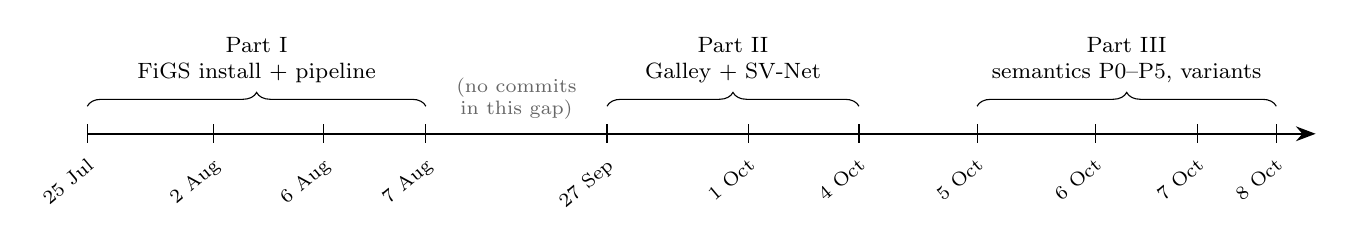
\begin{tikzpicture}[font=\small]
  \draw[thick, -{Stealth[length=2.5mm]}] (0,0) -- (15.6,0);
  \foreach \x/\d in {0/25 Jul, 1.6/2 Aug, 3.0/6 Aug, 4.3/7 Aug, 6.6/27 Sep, 8.4/1 Oct, 9.8/4 Oct, 11.3/5 Oct, 12.8/6 Oct, 14.1/7 Oct, 15.1/8 Oct}
    { \draw (\x,0.12) -- (\x,-0.12); \node[below, font=\scriptsize, rotate=40, anchor=north east] at (\x,-0.12) {\d}; }
  \draw[decorate, decoration={brace, amplitude=5pt}] (0,0.35) -- (4.3,0.35) node[midway, above=5pt, align=center, font=\footnotesize] {Part I\\FiGS install + pipeline};
  \draw[decorate, decoration={brace, amplitude=5pt}] (6.6,0.35) -- (9.8,0.35) node[midway, above=5pt, align=center, font=\footnotesize] {Part II\\Galley + SV-Net};
  \draw[decorate, decoration={brace, amplitude=5pt}] (11.3,0.35) -- (15.1,0.35) node[midway, above=5pt, align=center, font=\footnotesize] {Part III\\semantics P0--P5, variants};
  \node[font=\scriptsize, align=center, text=black!60] at (5.45,0.45) {(no commits\\in this gap)};
\end{tikzpicture}
\caption{Timeline of the work (not to scale). Laptop and SSD in July--August, intellisense05 in August, intellisense08
from late September.}
\label{fig:timeline}
\end{figure}

\begin{figure}[ht]
\centering
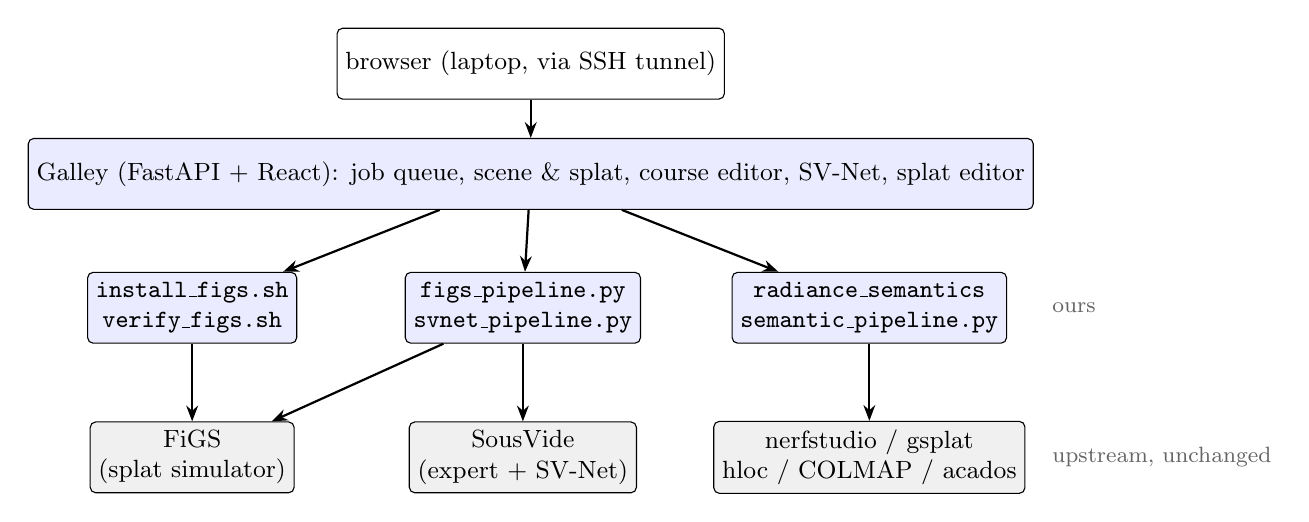
\begin{tikzpicture}[node distance=5mm and 6mm, font=\small,
  box/.style={draw, rounded corners=2pt, align=center, minimum height=9mm, inner sep=3pt, fill=white},
  up/.style={box, fill=gray!12}, ours/.style={box, fill=blue!8}, arr/.style={-{Stealth[length=2mm]}, thick}]
  \node[up] (fi) at (0,0) {FiGS\\(splat simulator)};
  \node[up] (sv) at (4.2,0) {SousVide\\(expert + SV-Net)};
  \node[up] (ns) at (8.6,0) {nerfstudio / gsplat\\hloc / COLMAP / acados};
  \node[ours] (inst) at (0,1.9) {\code{install\_figs.sh}\\\code{verify\_figs.sh}};
  \node[ours] (fp) at (4.2,1.9) {\code{figs\_pipeline.py}\\\code{svnet\_pipeline.py}};
  \node[ours] (sem) at (8.6,1.9) {\code{radiance\_semantics}\\\code{semantic\_pipeline.py}};
  \node[ours, minimum width=11.5cm] (gal) at (4.3,3.6) {Galley (FastAPI + React): job queue, scene \& splat, course editor, SV-Net, splat editor};
  \node[box] (br) at (4.3,5.0) {browser (laptop, via SSH tunnel)};
  \draw[arr] (br) -- (gal); \draw[arr] (gal) -- (inst); \draw[arr] (gal) -- (fp); \draw[arr] (gal) -- (sem);
  \draw[arr] (inst) -- (fi); \draw[arr] (fp) -- (sv); \draw[arr] (fp) -- (fi); \draw[arr] (sem) -- (ns);
  \node[font=\footnotesize, text=black!60, align=left, anchor=west] at (10.8,0) {upstream, unchanged};
  \node[font=\footnotesize, text=black!60, align=left, anchor=west] at (10.8,1.9) {ours};
\end{tikzpicture}
\caption{What was built around the upstream code. Grey: upstream (pinned, unchanged); blue: this project.}
\label{fig:layers}
\end{figure}

\begin{center}\small
\begin{tabular}{@{}>{\raggedright\arraybackslash}p{0.211\linewidth}>{\raggedright\arraybackslash}p{0.250\linewidth}>{\raggedright\arraybackslash}p{0.487\linewidth}@{}}
\toprule
\textbf{Machine} & \textbf{GPU} & \textbf{Role over time} \\
\midrule
dummy (home laptop, Ubuntu 24.04) & RTX 3050 Ti Laptop, 4 GB & July–Aug feasibility and first install; later the Galley build-and-test host \\
Portable SSD install & (host's GPU) & The whole environment on an SSD, mounted on other Ubuntu machines \\
intellisense05 (lab, campus-only) & RTX 2080, 8 GB & First complete capture-to-flight run (6 Aug) \\
intellisense08 (lab, Tailscale) & RTX 2080, 8 GB, 62 GB RAM, Ubuntu 22.04 & From 28 Sep: SV-Net host, then every semantics gate and experiment \\
RTX 5060 Ti PC (home) & 16 GB, Blackwell & Future main host (needs CUDA 12.8 / torch $\ge$ 2.7) \\
\bottomrule
\end{tabular}
\end{center}
\section{Getting FiGS to run (25 Jul – 7 Aug)}
\subsection{Feasibility check on the 4 GB laptop (25 Jul)}
\textbf{What we did.} Read the SOUS-VIDE paper and the three upstream repos (FiGS, FiGS-Examples, SousVide). Checked the laptop: RTX 3050 Ti 4 GB, driver 570 (CUDA 12.8), 16 GB RAM, Ubuntu 24.04. The upstream environment needs Python 3.10, torch 2.1.2 with its own conda CUDA 11.8 toolkit, tiny-cuda-nn built from source, nerfstudio 1.1.4 (with gsplat), COLMAP, acados (built with cmake) and hloc.

\textbf{Main risk identified.} Splat training (splatfacto) was thought to need about 6 GB of VRAM, more than the card had. Plan: use the laptop for simulation and test training later at reduced settings.

\textbf{Problems and fixes.}

\begin{center}\small
\begin{tabular}{@{}>{\raggedright\arraybackslash}p{0.162\linewidth}>{\raggedright\arraybackslash}p{0.370\linewidth}>{\raggedright\arraybackslash}p{0.415\linewidth}@{}}
\toprule
\textbf{Problem} & \textbf{Cause} & \textbf{Fix} \\
\midrule
conda not installed & fresh machine & installed Miniconda \\
tiny-cuda-nn build: \code{pkg\_\allowbreak{}resources} missing & pip's build isolation pulled a new setuptools & \code{pip install "setuptools<81"} and \code{-{}-no-build-isolation} \\
tiny-cuda-nn build used the wrong compiler & system nvcc 12.8 ahead of conda's CUDA 11.8 on PATH; then CUDA 11.8 rejected Ubuntu 24.04's GCC 13 & put \code{\$CONDA\_\allowbreak{}PREFIX/\allowbreak{}bin} first, \code{CUDA\_\allowbreak{}HOME=\$CONDA\_\allowbreak{}PREFIX}, install \code{gcc-11}/\code{g++-11} and use them as \code{CC}/\code{CXX} \\
example splats would not download & Google Drive's per-file quota on the shared academic link & downloaded in the browser, copied with \code{scp} (5 GB: backroom, flightroom, mid\_gate, src\_open) \\
example notebook asked for a missing scene & default \code{button} scene not in the download & pointed it at \code{backroom} + \code{circuit} (the paper's cluttered trajectory) \\
\bottomrule
\end{tabular}
\end{center}
\textbf{Result.} The example flight (backroom + circuit) ran headless with 0 failing cells and produced a rendered video; VRAM returned to idle. Simulation fits easily in 4 GB.

\subsection{A clean rebuild with an install script (2 Aug)}
\textbf{What we did.} Wrote \code{setup\_\allowbreak{}scripts/\allowbreak{}install\_\allowbreak{}figs.sh} (step-addressable, resumable, logs per step, \code{-{}-redo <step>}) and \code{verify\_\allowbreak{}figs.sh}, and rebuilt the environment with them. Verification: 22 passed, 0 failed. Measured: backroom/circuit flight 40 s, peak 608 MiB; tiny-cuda-nn build 2 min 29 s for one architecture.

\textbf{Problems and fixes — four host faults that cost most of a day.}

\begin{center}\small
\begin{tabular}{@{}>{\raggedright\arraybackslash}p{0.253\linewidth}>{\raggedright\arraybackslash}p{0.437\linewidth}>{\raggedright\arraybackslash}p{0.258\linewidth}@{}}
\toprule
\textbf{Problem} & \textbf{Cause} & \textbf{Fix} \\
\midrule
\code{nvidia-smi}: cannot communicate with the driver & an unattended upgrade installed kernel 7.0; the 570 driver's DKMS module builds only for 6.17. \code{GRUB\_\allowbreak{}DEFAULT=saved} + \code{GRUB\_\allowbreak{}SAVEDEFAULT=true} is not a pin: one boot into 7.0 made it sticky & pin GRUB to an explicit menuentry ID of 6.17.0-35, \code{GRUB\_\allowbreak{}SAVEDEFAULT=false}, \code{grub-editenv - unset saved\_\allowbreak{}entry} \\
driver installed but \code{Key was rejected by service} & Secure Boot with the DKMS signing key not enrolled & \code{mokutil -{}-import} and enrolment at the MOK screen on reboot (needs physical access) \\
install truncated mid-way & the desktop suspended the machine when idle & masked \code{sleep/\allowbreak{}suspend/\allowbreak{}hibernate} targets; lid and idle actions ignored \\
machine hard-locked during a JIT compile & ninja ran one \code{nvcc} per thread: 20 threads $\times$ 1–2 GB > 16 GB RAM + swap & \code{MAX\_\allowbreak{}JOBS=4} baked into \code{figs\_\allowbreak{}env.sh}; recovery needed Magic SysRq \\
two versions of nerfstudio and gsplat at once; gsplat compiled an orphaned \code{sh.cu} (\code{DEVICE\_\allowbreak{}GUARD} undefined) & the interrupted pip install left both \code{dist-info} directories & hard purge of both, reinstall; a duplicate-distribution check added \\
preflight error \code{NVIDIA: unbound variable} & the script tested that \code{nvidia-smi} exists, not that it runs, and fed its error text into arithmetic & detect ``installed but not communicating'' and print the remedy \\
\bottomrule
\end{tabular}
\end{center}
\textbf{Pinned versions} (drift was observed and corrected): nerfstudio 1.1.4 (1.1.5 pulls an incompatible gsplat), gsplat 1.0.0, torch 2.1.2 / torchvision 0.16.2 (every compiled extension is built against this ABI), numpy 1.26.4 (numpy 2 breaks the C ABI).

\subsection{A portable install on an SSD}
\textbf{What we did.} Put the whole environment (conda, the \code{kitchen} env with its CUDA 11.8, SousVide, acados, splats) on an external SSD so other lab machines could use it (\code{README\_\allowbreak{}PORTABLE.md}).

\textbf{Problems and fixes.} Conda environments are not relocatable (absolute paths in shebangs and \code{.pth} files), and Ubuntu mounts drives under \code{/\allowbreak{}media/\allowbreak{}<user>/\allowbreak{}<UUID>}, so the path changes with the user $\rightarrow$ mount explicitly at the original path by UUID; the installer detects a mismatch. The NVIDIA driver and apt packages belong to the host; tiny-cuda-nn is compiled for one GPU architecture and must be rebuilt for another (15–40 min); the environment needs the same or a newer Ubuntu (glibc).

\subsection{First complete capture-to-flight on the lab machine (6 Aug, intellisense05)}
\textbf{What we did.} Installed in place on intellisense05 (RTX 2080 8 GB, \code{TCNN\_\allowbreak{}CUDA\_\allowbreak{}ARCHITECTURES=75}) and ran our own capture end to end: a Samsung S23 4K60 HEVC video (191.7 s, 3.0 GB) with an 18 cm ArUco marker, transcoded to 1080p30, 300 frames, hloc SuperPoint + SuperGlue, COLMAP, ArUco metric alignment, splatfacto 30k steps, then a simulated flight.

\begin{center}\small
\begin{tabular}{@{}ll@{}}
\toprule
\textbf{Result} & \textbf{Value} \\
\midrule
Registration & 300 / 300 images, 40,542 points, reprojection error 1.43 px \\
SuperGlue matching & 38 min (44,850 exhaustive pairs) \\
Splat training & 34 min, peak 5,203 MiB \\
Flight simulation & 51 s for 16 s of flight, peak 635 MiB \\
Whole pipeline & about 1 h 40 min \\
\bottomrule
\end{tabular}
\end{center}
\textbf{Problems and fixes.}

\begin{center}\small
\begin{tabular}{@{}>{\raggedright\arraybackslash}p{0.266\linewidth}>{\raggedright\arraybackslash}p{0.381\linewidth}>{\raggedright\arraybackslash}p{0.301\linewidth}@{}}
\toprule
\textbf{Problem} & \textbf{Cause} & \textbf{Fix} \\
\midrule
install and verify scripts said a healthy install was missing & default prefix \code{\textasciitilde{}/\allowbreak{}projects/\allowbreak{}figs\_\allowbreak{}validation} hard-coded & \code{-{}-prefix} every time; later scripts resolve the project root themselves \\
\code{import\_\allowbreak{}images(): incompatible function arguments} & pycolmap 4.1.1 renamed \code{image\_\allowbreak{}list} to \code{image\_\allowbreak{}names}; hloc still used the old name & one-line patch in the hloc submodule (later applied automatically by the pipeline's \code{patch} step) \\
\code{DataLoader worker … Segmentation fault} at 0/300 & OpenCV 5.0.0 inside forked DataLoader workers & \code{num\_\allowbreak{}workers=0} in hloc's feature extraction (patched automatically) \\
\code{libqpOASES\_\allowbreak{}e.so: cannot open shared object file} in \code{Simulator()} (\code{docs/\allowbreak{}errors.txt}) & the environment was activated with \code{conda activate} only; \code{LD\_\allowbreak{}LIBRARY\_\allowbreak{}PATH} and \code{ACADOS\_\allowbreak{}SOURCE\_\allowbreak{}DIR} come from \code{figs\_\allowbreak{}env.sh} & always \code{source figs\_\allowbreak{}env.sh}; preflight now loads the library by soname in the first seconds \\
drone flew ``below the floor'', video looked like mush & course files are z-down and y-negated relative to \code{transforms.json}: course = (x, $-$y, $-$z) & derived and documented the conversion; every waypoint is validated against the captured volume \\
\code{ns-viewer} held \textasciitilde{}4.6 GB & left running & close it before training \\
CasADi 3.7.2 newer than acados supports & unpinned & works; noted as first suspect if codegen breaks \\
marker detections clustered in time & most marker frames in the first 20 s & \code{num\_\allowbreak{}marked} raised from 20 to 40 so the late window contributes \\
\bottomrule
\end{tabular}
\end{center}
\subsection{One resumable pipeline script (7 Aug)}
\begin{figure}[ht]
\centering
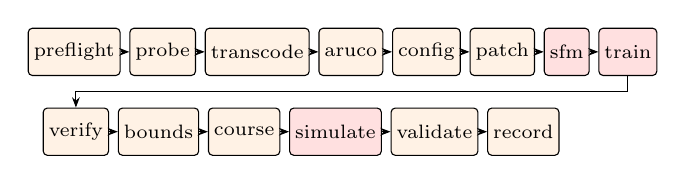
\begin{tikzpicture}[font=\scriptsize, node distance=1.1mm,
  s/.style={draw, rounded corners=1.5pt, fill=orange!10, minimum height=6mm, inner sep=2pt},
  g/.style={s, fill=red!12}]
  \node[s] (a) {preflight}; \node[s, right=of a] (b) {probe}; \node[s, right=of b] (c) {transcode};
  \node[s, right=of c] (d) {aruco}; \node[s, right=of d] (e) {config}; \node[s, right=of e] (f) {patch};
  \node[g, right=of f] (g1) {sfm}; \node[g, right=of g1] (g2) {train};
  \node[s, below=4mm of a, anchor=north west, xshift=-4mm] (h) {verify}; \node[s, right=of h] (i) {bounds};
  \node[s, right=of i] (j) {course}; \node[g, right=of j] (k) {simulate}; \node[s, right=of k] (l) {validate};
  \node[s, right=of l] (m) {record};
  \foreach \u/\v in {a/b,b/c,c/d,d/e,e/f,f/g1,g1/g2,h/i,i/j,j/k,k/l,l/m} \draw[-{Stealth[length=1.3mm]}] (\u) -- (\v);
  \draw[-{Stealth[length=1.3mm]}] (g2.south) |- ($(h.north)+(0,0.2)$) -- (h.north);
\end{tikzpicture}
\caption{The pipeline's steps (the \code{gsplat} step was split into \code{sfm} + \code{train} on 27 Sep). Red: GPU
steps. Each step leaves a marker with a fingerprint of its inputs, so a re-run resumes after the last finished step.}
\end{figure}

\textbf{What we did.} Replaced the notebook with \code{figs/\allowbreak{}figs\_\allowbreak{}pipeline.py}: steps \code{preflight → probe → transcode → aruco → config → patch → gsplat → verify → bounds → course → simulate → validate → record}, state on disk (an interrupt costs one step), VRAM sampling, an ArUco time histogram, and a table of known failure modes printed with their remedy. First commit of this repository (35efbad): ``validated end to end on an RTX 2080: 300/300 frames registered, 5,203 MiB peak training VRAM, \textasciitilde{}1 h 40 m''.

\textbf{Quiet failures the script exists to catch}: a wrong marker length (a perfectly reconstructed room at the wrong scale), a wrong marker ID (alignment fails an hour later), partial registration, waypoints outside the captured volume.

\section{Galley, the web console (27 Sep – 4 Oct)}
Galley is a FastAPI + React console in \code{ui/\allowbreak{}} that drives the pipeline scripts. Design rule: the scripts stay the source of truth; Galley only chooses flags and step ranges and reads the scripts' state files, so anything started in the browser can be resumed from the shell. Work in this period was written by Claude in a cloud sandbox; Suhan committed, pulled on the hosts, ran gate scripts and pasted the logs back.

\subsection{Galley phases 0–3 (built in the cloud, gated on dummy, committed 27 Sep)}
\begin{figure}[ht]
\centering
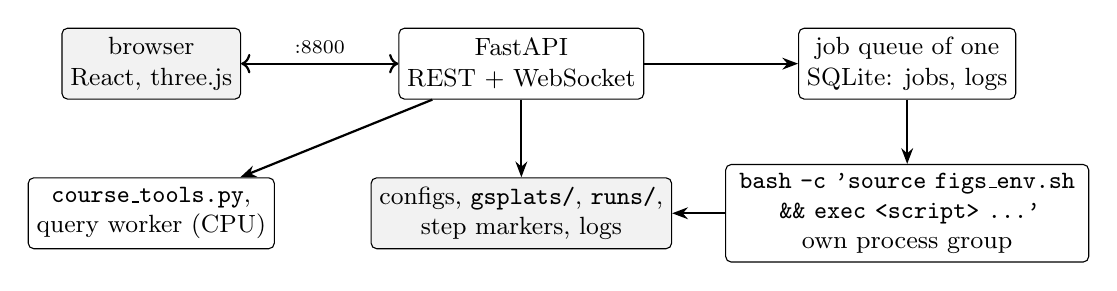
\begin{tikzpicture}[font=\small, node distance=5mm and 7mm,
  box/.style={draw, rounded corners=2pt, align=center, minimum height=9mm, inner sep=3pt, fill=white},
  arr/.style={-{Stealth[length=2mm]}, thick}]
  \node[box, fill=gray!10] (br) at (0,0) {browser\\React, three.js};
  \node[box] (api) at (4.7,0) {FastAPI\\REST + WebSocket};
  \node[box] (q) at (9.6,0) {job queue of one\\SQLite: jobs, logs};
  \node[box, text width=4.4cm] (w) at (9.6,-1.9) {\code{bash -c 'source figs\_env.sh \&\& exec <script> \dots'}\\own process group};
  \node[box, fill=gray!10] (st) at (4.7,-1.9) {configs, \code{gsplats/}, \code{runs/},\\step markers, logs};
  \node[box] (tools) at (0,-1.9) {\code{course\_tools.py},\\query worker (CPU)};
  \draw[arr, <->] (br) -- node[above, font=\scriptsize] {:8800} (api);
  \draw[arr] (api) -- (q); \draw[arr] (q) -- (w); \draw[arr] (w) -- (st); \draw[arr] (api) -- (st);
  \draw[arr] (api) -- (tools);
\end{tikzpicture}
\caption{Galley's architecture. The scripts remain the source of truth: Galley builds validated argument lists, runs one
GPU job at a time, and reads the scripts' state files.}
\end{figure}

\begin{center}\small
\begin{tabular}{@{}>{\raggedright\arraybackslash}p{0.096\linewidth}>{\raggedright\arraybackslash}p{0.472\linewidth}>{\raggedright\arraybackslash}p{0.380\linewidth}@{}}
\toprule
\textbf{Phase} & \textbf{What it added} & \textbf{Gate result} \\
\midrule
0 & dummy aligned with the lab setup & backroom + circuit flown by \code{figs\_\allowbreak{}pipeline.py}: 34 s, tracking max 0.034 m, 614 MiB \\
1 & backend core: SQLite job queue of one, config models, log streaming over WebSocket, cancel by process group & 26 tests, a real preflight job through the queue, cancel of a running job \\
2 & Scene \& Splat page; the pipeline's \code{gsplat} step split into \code{sfm} + \code{train} & retrain from the UI, training curve shown, previous model promoted back, flight re-run \\
3 & course editor: 3D waypoints over the SfM points, MinTimeSnap preview, clearance, Save and fly & a browser-built course passes \code{course} and flies (tracking max 0.069 m) \\
\bottomrule
\end{tabular}
\end{center}
\textbf{Problems and fixes.}

\begin{center}\small
\begin{tabular}{@{}>{\raggedright\arraybackslash}p{0.190\linewidth}>{\raggedright\arraybackslash}p{0.308\linewidth}>{\raggedright\arraybackslash}p{0.450\linewidth}@{}}
\toprule
\textbf{Problem} & \textbf{Cause} & \textbf{Fix} \\
\midrule
the known-good backroom + circuit was refused by the \code{course} step & a \code{null} (free) waypoint cell became NaN & check only constrained axes \\
\code{simulate} failed writing the video & imageio's FFMPEG writer refuses a \code{.partial} extension (ffmpeg likewise in \code{transcode}) & write \code{<scene>\_\allowbreak{}flight.partial.mp4}, rename; \code{-f mp4} \\
a retrain repeated SfM (\textasciitilde{}45 min) & one \code{gsplat} step & split into \code{sfm} (upstream \code{generate\_\allowbreak{}gsplat} with its \code{ns-train} call intercepted) and \code{train} \\
preflight warned ``under 6 GB, training will OOM'' & wrong assumption & measured: with \code{-{}-cache-images cpu}, backroom trains on the 4 GB laptop at \textbf{2,360 MiB} (60 min); most of the 5.2 GB reference was images cached on the GPU \\
editing a course under the same name kept the old flight & step fingerprints did not include the course file & fingerprints include a course digest \\
a course saved from the browser flew a different path & browsers write 0.0 as \code{0}; FiGS's \code{KF\_\allowbreak{}to\_\allowbreak{}TpFO} reads an integer cell as the previous cell's value, silently & Galley writes floats; the \code{course} step refuses integer cells; a lint endpoint finds them \\
clearance put the known-good circuit 2.7 cm from an obstacle & isolated SfM outlier points & clearance = distance to the 5th-nearest sparse point \\
stretching keyframe times did not slow the flight & the expert's \code{kT} makes MinTimeSnap re-optimise durations; file times are only a starting guess & \emph{Re-time like expert} preview and \emph{Write solved times} \\
\bottomrule
\end{tabular}
\end{center}
\subsection{SV-Net through Galley (27 Sep – 1 Oct)}
\textbf{What we did.} \code{figs/\allowbreak{}svnet\_\allowbreak{}pipeline.py} reproduces the upstream SOUS-VIDE notebook step for step (\code{preflight → rollout → observe → train\_\allowbreak{}hist → train\_\allowbreak{}comm → deploy}), calling upstream code unchanged, resumable per cohort, plus SV-Net pages in Galley.

\textbf{Problems and fixes.}

\begin{center}\small
\begin{tabular}{@{}>{\raggedright\arraybackslash}p{0.201\linewidth}>{\raggedright\arraybackslash}p{0.364\linewidth}>{\raggedright\arraybackslash}p{0.383\linewidth}@{}}
\toprule
\textbf{Problem} & \textbf{Cause} & \textbf{Fix} \\
\midrule
commNet out of memory in epoch 2 on the 4 GB laptop & every step in one process: the splat, observation tensors and PyTorch's cache stayed on the card & one child process per step; \code{gc.collect()} + \code{empty\_\allowbreak{}cache()} after deploy; test pass without autograd \\
no progress in logs & rich progress bars draw nothing when stdout is a pipe & plain progress lines and per-epoch losses in \code{live\_\allowbreak{}*.jsonl} \\
a smaller re-run mixed old and new rollouts & upstream overwrites by index & old data archived before a re-run \\
a second \code{train\_\allowbreak{}hist} continued the first & \code{Pilot()} loads the network on disk & \code{-{}-fresh histNet} or \code{-{}-fresh commNet} \\
upstream's tracking error looked fine for bad flights & \code{compute\_\allowbreak{}flight\_\allowbreak{}metrics} uses \code{axis=0} (the whole path per axis), not the distance to each point & our per-point tracking error reported next to upstream's \\
commNet needs \textasciitilde{}6.8 GB with in-loop evaluation & training + the splat for evaluation flights & SV-Net moved to intellisense08 (8 GB) \\
\bottomrule
\end{tabular}
\end{center}
\textbf{Lab bring-up (28 Sep – 1 Oct).} \code{ui/\allowbreak{}deploy/\allowbreak{}host.sh} (paths by hostname), \code{bringup.sh}, a machine profile \code{ui/\allowbreak{}machines/\allowbreak{}intellisense08.toml}; the repository moved to the Radiance-ICE-22 organisation (\code{Radiance-Environment-Setup}). verify 21/21; backroom + circuit identical to dummy (tracking max 0.034 m).

\textbf{Gate result (1 Oct, 49 min, cohort \code{p4\_\allowbreak{}smoke}).} Every step ran through the queue; commNet peaked at 6,785 MiB. The expert tracks the course to 1.7 cm; \textbf{the student (Maverick) does not fly it} (mean 9.4 m off, 16 \% within 0.3 m). Next for SV-Net: watch its video, then a larger dataset (\code{data\_\allowbreak{}beta}). Still open.

\subsection{Console features and the Windows 7 ribbon redesign (1 – 4 Oct)}
\begin{itemize}
  \item \textbf{Drone model (1 Oct):} the team's CAD (1.62 M triangles) converted to a 159k-triangle GLB in FiGS's body frame; measured bounding sphere 0.19 m; clearance now reports the \emph{gap} (centre distance minus 0.19 m), default minimum 0.15 m.
  \item \textbf{\code{run\_\allowbreak{}ui.sh} (1 Oct):} start/stop/status per host; refuses to stop while a job runs (a stopped server orphans the job).
  \item \textbf{Ribbon redesign (1 Oct):} designed in Figma (design system, ribbons, five screens), then built into the frontend: ribbon with hover help for every command, Explorer, tabbed documents, Properties, Output, status bar, shortcuts. Problems: Figma's Starter plan allows 3 pages and 20 MCP calls a month $\rightarrow$ screens generated by a local Figma plugin; Noto Sans lacks $\rightarrow$, $\le$ and box glyphs $\rightarrow$ reworded.
  \item \textbf{3–4 Oct:} full screen, resizable tiles; a stale \code{index.html} after deploys $\rightarrow$ served with no-cache, plus a ``newer build'' notice and an end to an endless ``Loading the 3D editor''.
  \item \textbf{Splat in the course editor (4 Oct):} the checkpoint exported to the 32-byte \code{.splat} format (cached, keyed by run + checkpoint + mtime); drei's loader flips (x, y, z) $\rightarrow$ (x, $-$y, $-$z), which is exactly splat $\rightarrow$ course. Arrow-key flying.
  \item \textbf{Video upload and Google Drive import (4 Oct):} resumable chunked uploads; from home the upload crawled at \textasciitilde{}0.5 MB/s (Tailscale relaying through DERP Bangalore) $\rightarrow$ the host downloads picked files directly from Google Drive (OAuth \code{drive.file}, token in memory, Range resume, MD5 check).
  \item \textbf{A log with 90k lines (4 Oct):} \code{figs\_\allowbreak{}pipeline.sh()} read child output in text mode, turning every tqdm \code{\textbackslash{}r} redraw into a new line (hloc's matching stored \textasciitilde{}90k lines and looked stuck) $\rightarrow$ output passed as bytes; Galley updates a redrawn line in place.
\end{itemize}
\textbf{Workflow traps of this period:} git from the Cowork VM left lock files on the laptop repo; the laptop copy is CRLF; dummy diverged once because files were copied with \code{scp} ($\rightarrow$ \code{pull.ff only}, update only by pulling); \code{-{}-train-arg} needs the \code{=} form.

\section{Semantic goals (5 – 8 Oct)}
\begin{figure}[ht]
\centering
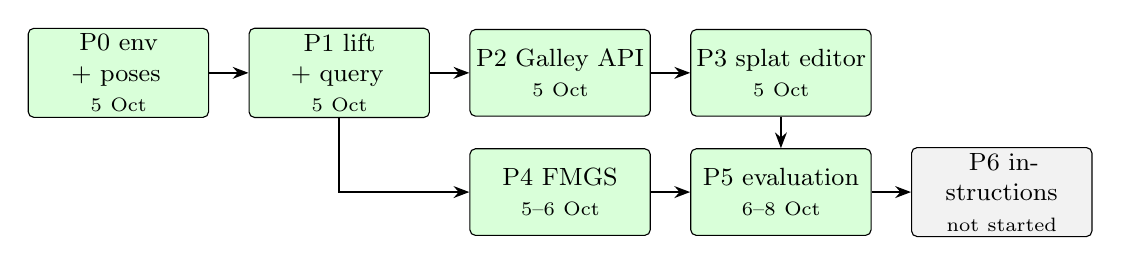
\begin{tikzpicture}[font=\small, node distance=4mm and 5mm,
  p/.style={draw, rounded corners=2pt, align=center, minimum height=11mm, text width=2.15cm, inner sep=2pt},
  arr/.style={-{Stealth[length=2mm]}, thick}]
  \node[p, fill=green!15] (p0) {P0 env + poses\\\scriptsize 5 Oct};
  \node[p, fill=green!15, right=of p0] (p1) {P1 lift + query\\\scriptsize 5 Oct};
  \node[p, fill=green!15, right=of p1] (p2) {P2 Galley API\\\scriptsize 5 Oct};
  \node[p, fill=green!15, right=of p2] (p3) {P3 splat editor\\\scriptsize 5 Oct};
  \node[p, fill=green!15, below=of p2] (p4) {P4 FMGS\\\scriptsize 5--6 Oct};
  \node[p, fill=green!15, right=of p4] (p5) {P5 evaluation\\\scriptsize 6--8 Oct};
  \node[p, fill=gray!10, right=of p5] (p6) {P6 instructions\\\scriptsize not started};
  \draw[arr] (p0) -- (p1); \draw[arr] (p1) -- (p2); \draw[arr] (p2) -- (p3);
  \draw[arr] (p1) |- (p4); \draw[arr] (p3) -- (p5); \draw[arr] (p4) -- (p5); \draw[arr] (p5) -- (p6);
\end{tikzpicture}
\caption{The semantics phases and their gates (green: passed).}
\end{figure}

\begin{figure}[ht]
\centering
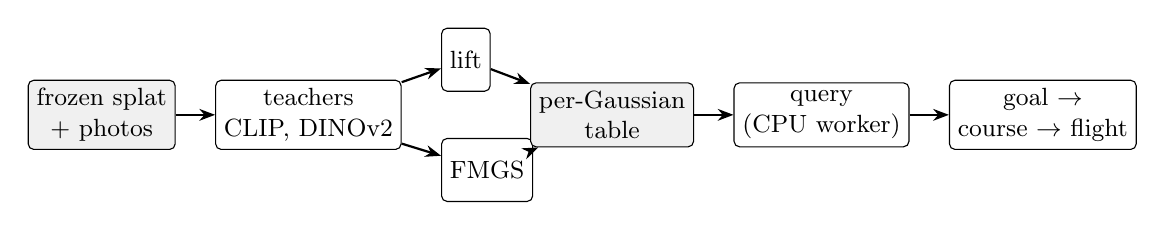
\begin{tikzpicture}[node distance=4mm and 5mm, font=\small,
  box/.style={draw, rounded corners=2pt, align=center, minimum height=8mm, inner sep=3pt, fill=white},
  arr/.style={-{Stealth[length=2mm]}, thick}]
  \node[box, fill=gray!12] (sp) {frozen splat\\+ photos};
  \node[box, right=of sp] (t) {teachers\\CLIP, DINOv2};
  \node[box, right=of t, yshift=7mm] (l) {lift};
  \node[box, right=of t, yshift=-7mm] (f) {FMGS};
  \node[box, fill=gray!12, right=of l, yshift=-7mm] (tab) {per-Gaussian\\table};
  \node[box, right=of tab] (q) {query\\(CPU worker)};
  \node[box, right=of q] (c) {goal $\rightarrow$\\course $\rightarrow$ flight};
  \draw[arr] (sp) -- (t); \draw[arr] (t) -- (l); \draw[arr] (t) -- (f); \draw[arr] (l) -- (tab); \draw[arr] (f) -- (tab);
  \draw[arr] (tab) -- (q); \draw[arr] (q) -- (c);
\end{tikzpicture}
\caption{The semantic layer in one line (details in \code{semantic\_embedding\_report.pdf}).}
\end{figure}

The plan (\code{SEMANTICS\_\allowbreak{}PLAN.md}) has seven phases, each closed by a gate on intellisense08: P0 environment and poses, P1 the training-free lift and a CLI query, P2 Galley's API and a CPU query worker, P3 a splat editor (query $\rightarrow$ course $\rightarrow$ flight), P4 the FMGS backend, P5 the evaluation, P6 instructions $\rightarrow$ courses $\rightarrow$ SV-Net.

\subsection{Phase 0 — environment and pose check (5 Oct)}
\textbf{What we did.} Package \code{radiance\_\allowbreak{}semantics}; \code{install\_\allowbreak{}semantics.sh} adds OpenCLIP and DINOv2 to \code{kitchen} without moving torch; probes for gsplat feature rendering; a camera check.

\textbf{Problems and fixes.}

\begin{center}\small
\begin{tabular}{@{}>{\raggedright\arraybackslash}p{0.221\linewidth}>{\raggedright\arraybackslash}p{0.365\linewidth}>{\raggedright\arraybackslash}p{0.362\linewidth}@{}}
\toprule
\textbf{Problem} & \textbf{Cause} & \textbf{Fix} \\
\midrule
newest OpenCLIP needs \code{timm>=1.0.17}; nerfstudio pins \code{timm==0.6.7} & version conflict & OpenCLIP pinned at 2.24.0 (timm optional), \code{huggingface\_\allowbreak{}hub<1} \\
a constraints file from \code{pip freeze} constrained nothing & conda packages appear as \code{name @ file:/\allowbreak{}/\allowbreak{}…}; in the cloud test env numpy 2.2 slipped in and torch broke (\code{\_\allowbreak{}ARRAY\_\allowbreak{}API not found}) & constraints built from package metadata; every install \code{-{}-no-deps} + constraints, torch re-checked \\
first gate: \code{Unsupported number of channels: 64} in \code{rasterize\_\allowbreak{}to\_\allowbreak{}pixels\_\allowbreak{}bwd} & gsplat 1.0.0's backward kernel takes $\le$ 32 channels (forward $\le$ 512) & \code{render\_\allowbreak{}features} splits grad-requiring features into 32-channel chunks (29 passes per image for the lift) \\
features would be projected through wrong cameras & splatfacto applies its learned pose correction only while training & \code{cameras.optimized\_\allowbreak{}c2w} applies it explicitly: \textbf{+4.22 dB PSNR} on backroom (31.68 vs 27.46 dB), corrections up to 39 mm / 2\textdegree{} \\
\bottomrule
\end{tabular}
\end{center}
Second gate (09:48): all five checks passed.

\subsection{Phase 1 — teachers, lift and query (5 Oct)}
\textbf{What we did.} \code{semantic\_\allowbreak{}pipeline.py} (resumable steps \code{preflight → cameras → teachers → lift → export}); CLIP crop pyramid (7 scales, averaged) and DINOv2 maps per photo; the blend-weighted lift onto 532,361 Gaussians; the table; \code{semantic\_\allowbreak{}query.py} with LERF relevancy and voxel clusters; five annotated development queries.

First gate (fc7aed2): teachers 31.5 min, lift 3 min 11 s (7.6 GB), 3 of 5 hits.

\begin{center}\small
\begin{tabular}{@{}>{\raggedright\arraybackslash}p{0.286\linewidth}>{\raggedright\arraybackslash}p{0.272\linewidth}>{\raggedright\arraybackslash}p{0.390\linewidth}@{}}
\toprule
\textbf{Problem} & \textbf{Cause} & \textbf{Fix} \\
\midrule
red tool chest missed by 1.3 m & our annotation was placed at the wrong depth & Suhan re-placed it from the splat \\
whiteboard: 75,596 Gaussians selected, 10 m clusters & a fixed 0.55 floor lets every white wall and ceiling in & \textbf{relative threshold} $\tau$ = 0.55 + 0.5$\cdot$(peak $-$ 0.55), peak = mean of the top 100 \\
lift peak 7.6 GB & the full 512-channel CLIP map upsampled at once & upsample per 32-channel chunk \\
10,741 ``seen'' Gaussians in the lift vs 11,592 in the table & weights in (0, 1e-8] & unseen means weight exactly 0, everywhere \\
\bottomrule
\end{tabular}
\end{center}
Second gate (16:12): \textbf{5 of 5}, mean error 0.23 m. The five queries had shaped the threshold, so they became a development set; the evaluation would need a separate frozen set.

\subsection{Phase 2 — Galley backend and query worker (5 Oct)}
\textbf{What we did.} A long-lived CPU-only query worker (\code{semantic\_\allowbreak{}worker.py}, JSON lines; keeps the CLIP text tower and memory-mapped tables), Galley's client and the semantics API. Stale tables are detected by the same key as Galley's \code{.splat} cache.

\begin{center}\small
\begin{tabular}{@{}>{\raggedright\arraybackslash}p{0.248\linewidth}>{\raggedright\arraybackslash}p{0.496\linewidth}>{\raggedright\arraybackslash}p{0.203\linewidth}@{}}
\toprule
\textbf{Problem} & \textbf{Cause} & \textbf{Fix} \\
\midrule
one backend test failed only on the host (405 instead of 404) & httpx normalised \code{/\allowbreak{}api/\allowbreak{}scenes/\allowbreak{}../\allowbreak{}semantics/\allowbreak{}query}; with a built frontend present the path fell through to the static mount & the test uses a scene name the route rejects (400) \\
\bottomrule
\end{tabular}
\end{center}
Gate: cold query 5.8 s, warm 716–789 ms, 5/5 hits — identical to the CLI.

\subsection{Phase 3 — the splat editor (5 Oct)}
\textbf{What we did.} \code{\#/\allowbreak{}splat/\allowbreak{}<scene>}: the splat rendered in the browser (renderer vendored from drei with a recolour path), relevancy heatmap, candidates, picking, annotations, and \textbf{Send to course} (the approach point becomes the final keyframe, yaw facing the object).

\begin{center}\small
\begin{tabular}{@{}>{\raggedright\arraybackslash}p{0.391\linewidth}>{\raggedright\arraybackslash}p{0.454\linewidth}>{\raggedright\arraybackslash}p{0.103\linewidth}@{}}
\toprule
\textbf{Problem} & \textbf{Cause} & \textbf{Fix} \\
\midrule
a lone candidate showed ``runner-up at 100 \%'' & the UI misread the margin (top $-$ runner-up)/top & text fixed \\
a contextual ribbon tab reset to Home & a lazily loaded document registered after the reset & ribbon fix \\
\bottomrule
\end{tabular}
\end{center}
Gate: ``red tool chest'' $\rightarrow$ course $\rightarrow$ flight (tracking max 8 mm); browser half: the whiteboard sent from the editor and flown (tracking max 73 mm); recolouring 532k Gaussians in 20 ms + 71 ms.

\subsection{Phase 4 — FMGS on a frozen splat (5 – 6 Oct)}
\begin{figure}[ht]
\centering
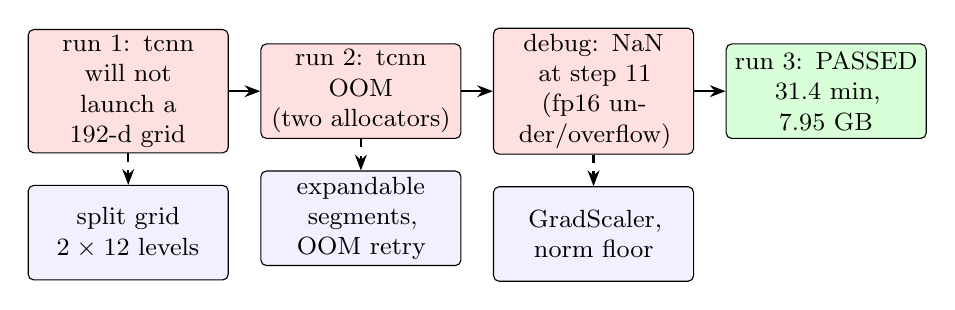
\begin{tikzpicture}[font=\small, node distance=4mm and 4mm,
  r/.style={draw, rounded corners=2pt, align=center, minimum height=12mm, text width=2.4cm, inner sep=2pt},
  arr/.style={-{Stealth[length=2mm]}, thick}]
  \node[r, fill=red!12] (r1) {run 1: tcnn will not\\launch a 192-d grid};
  \node[r, fill=red!12, right=of r1] (r2) {run 2: tcnn OOM\\(two allocators)};
  \node[r, fill=red!12, right=of r2] (r3) {debug: NaN at step 11\\(fp16 under/overflow)};
  \node[r, fill=green!15, right=of r3] (r4) {run 3: PASSED\\31.4 min, 7.95 GB};
  \node[r, below=of r1, fill=blue!6] (x1) {split grid\\$2\times12$ levels};
  \node[r, below=of r2, fill=blue!6] (x2) {expandable segments,\\OOM retry};
  \node[r, below=of r3, fill=blue!6] (x3) {GradScaler,\\norm floor};
  \draw[arr] (r1) -- (r2); \draw[arr] (r2) -- (r3); \draw[arr] (r3) -- (r4);
  \draw[arr, dashed] (r1) -- (x1); \draw[arr, dashed] (r2) -- (x2); \draw[arr, dashed] (r3) -- (x3);
\end{tikzpicture}
\caption{The Phase 4 gate: three failures, each with its fix, before the pass.}
\end{figure}

\textbf{What we did.} A standalone FMGS trainer (decided over an \code{ns-train} plugin: the splat is frozen, so only cameras and teacher maps are needed, and it shares the lift's cameras and renderer for a fair comparison): hash-grid feature field, CLIP and DINO heads, CLIP Huber + DINO L2 + pixel-alignment loss, 4,200 steps; bake to the same table; View $\triangleright$ Compare in the editor.

\begin{center}\small
\begin{tabular}{@{}>{\raggedright\arraybackslash}p{0.094\linewidth}>{\raggedright\arraybackslash}p{0.124\linewidth}>{\raggedright\arraybackslash}p{0.384\linewidth}>{\raggedright\arraybackslash}p{0.321\linewidth}@{}}
\toprule
\textbf{Gate run} & \textbf{Problem} & \textbf{Cause} & \textbf{Fix} \\
\midrule
1 (73e7968) & tiny-cuda-nn \code{invalid configuration argument} & on sm\_75 any 192-dim hash grid fails to launch (every grid $\le$ 96 dims runs) — a width limit, not memory & \code{fmgs/\allowbreak{}diag.py} probes; the 24 levels built as \textbf{two 12-level grids} (16$\rightarrow$84, 98$\rightarrow$512; every level within 1 \%); per-part PyTorch fallback \\
2 (70d2178) & \code{cuMemCreate … CUDA\_\allowbreak{}ERROR\_\allowbreak{}OUT\_\allowbreak{}OF\_\allowbreak{}MEMORY} in tcnn's backward & live tensors peaked at 5.9 GB, but PyTorch's cache kept 1–3 GB of fragmented free blocks that tcnn's own allocator cannot use; the OOM ladder caught only \code{torch.cuda.OutOfMemoryError} & expandable segments; tcnn's \code{RuntimeError} recognised; a failed step retried once; shorter tensor lifetimes \\
(debug) & loss NaN at step 11 & CLIP gradients (\textasciitilde{}1e-8) underflowed in tcnn's fp16 before its $\times$128 loss scale; pixel alignment normalised \textasciitilde{}0 vectors, gradients 2.25e4 overflowed & dynamic loss scaling (GradScaler); 1e-3 norm floor in pixel alignment \\
3 (7344e7a) & — & — & \textbf{PASSED} 6 Oct 13:31: 4,200 steps in 31.4 min, peak 5.5 GB PyTorch / 7.95 GB device, Gaussians and checkpoint unchanged; dev queries FMGS 4/5, lift 5/5 \\
\bottomrule
\end{tabular}
\end{center}
\textbf{Hand-off to Claude Code on the host (6 Oct).} From here Claude ran directly on intellisense08 (tests, probes, gates, logs), guided by \code{CLAUDE.md}. Gate run 2's diagnosis and the fixes above were the first work done that way. pytest was added to \code{kitchen} with \code{-{}-no-deps} and the frozen constraints; 68 semantics tests pass.

\subsection{Phase 5 — evaluation on two scenes (6 Oct)}
\textbf{What we did.} Four variants — L-C (lift, CLIP query), L-CD (lift + DINO at query time: diffusion over a DINO-weighted kNN graph and a DINO split of merged candidates), F-C (FMGS on CLIP alone), F-CD (FMGS with its paper losses) — on two scenes; an evaluator (multi-instance hits, failure kinds, absent-object false positives and AUROC); query sets annotated from photos and frozen before any result (f38225b: backroom 13 + 3 absent, flightroom 16 + 3).

\begin{center}\small
\begin{tabular}{@{}>{\raggedright\arraybackslash}p{0.188\linewidth}>{\raggedright\arraybackslash}p{0.378\linewidth}>{\raggedright\arraybackslash}p{0.383\linewidth}@{}}
\toprule
\textbf{Problem} & \textbf{Cause} & \textbf{Fix} \\
\midrule
GTN\_lab\_v1 looked non-metric (camera path 1,309 m, bounds $\pm$168 m) & scale was right (marker check: median ratio 1.003); 3 of 600 cameras registered 100–219 m away & \code{pose\_\allowbreak{}inliers} drops cameras > 4 $\times$ the p90 distance from the median \\
GTN\_lab\_v1's room is folded & SfM fused two walls with the same logo (a ``doppelganger'' failure); 395 of 600 cameras face one direction; HDR footage without tone mapping (18 dB PSNR) & second scene changed to \textbf{flightroom} (mocap poses); GTN workspace deleted at Suhan's request, video kept \\
intellisense\_v1 failed in SfM alignment & no ArUco marker visible in the footage & capture deleted; re-shoot with the marker needed \\
annotations from sparse SfM points leaked to the background on thin objects & few points on monitors, tripods, chairs & \code{locate -{}-depth}: picks from the splat's rendered depth \\
host reset twice mid-training (17:47, \textasciitilde{}18:14) & lightning power cuts & FMGS checkpoints every 1,000 steps; jobs resumed from step 3,000; GPU telemetry logging added for the diagnosis and removed afterwards at Suhan's request \\
evaluation reported the wrong build time for resumed runs & only the last leg was timed & build time = steps ÷ it/s \\
the expert flew a semantic course at 33 m/s, 528 \% thrust & the editor's \emph{Add} halved a leg's time; MinTimeSnap (SLSQP on raw durations) stalls at a badly squeezed guess and reports success & \emph{Add} inserts time (distance ÷ mean speed); fast legs flagged in the editor, lint and the \code{course} step; a stalled re-time is reported \\
the editor scored only one instance and no absent objects & written for the dev set & multi-instance and negative scoring like the evaluator \\
the frontend could not be rebuilt on the host & no Node.js, no sudo & Node 22.23.3 under \code{\textasciitilde{}/\allowbreak{}Radiance/\allowbreak{}tools} \\
\bottomrule
\end{tabular}
\end{center}
\textbf{Results (frozen sets).} Lift 8/13 and 10/16 ($\approx$ 0.62), \textasciitilde{}0.2 m median error; F-C 6/13, 8/16; F-CD 7/13, 4/16 — F-CD's CLIP channel fragmented into tiny clusters (DINO dominates its loss). The relevancy floor is the only query setting that moves hits; the lift's render width (480/720/960 px) changes nothing. Also written: a backend implementation report.

\subsection{Why the misses? Diagnostic and ground-truth check (7 Oct)}
\textbf{What we did.} \code{diag\_\allowbreak{}teachers.py} measured relevancy at three stages per object: lifting into 3D loses \textasciitilde{}0.007; averaging the crop scales costs 0.07–0.09; several misses are CLIP recognition limits. Then every miss was re-examined in the photos.

\begin{center}\small
\begin{tabular}{@{}>{\raggedright\arraybackslash}p{0.202\linewidth}>{\raggedright\arraybackslash}p{0.398\linewidth}>{\raggedright\arraybackslash}p{0.349\linewidth}@{}}
\toprule
\textbf{Problem} & \textbf{Cause} & \textbf{Fix} \\
\midrule
purple foam mat ``wrong object'' & our annotation had leaked 2 m behind the mat; the model was right & re-placed from splat depth (amended set; frozen set kept) \\
glass door cabinet ``wrong object'' & the upper glass cabinets were not annotated as instances & instances added \\
\bottomrule
\end{tabular}
\end{center}
backroom lift 8/13 $\rightarrow$ 10/13 on the amended set.

\subsection{Teacher variants A, B, C (7 – 8 Oct)}
\textbf{What we did.} Variant plumbing (\code{-{}-clip-mode/\allowbreak{}-{}-clip-model/\allowbreak{}-{}-table-suffix}, tables record their CLIP model), then three branches: \textbf{A} multi-scale CLIP (three scale groups, chosen per query), \textbf{B} CLIP on SAM segments, \textbf{C} ViT-L/14. Each rebuilt on both scenes for lift, F-C and F-CD (long runs in tmux).

\begin{center}\small
\begin{tabular}{@{}>{\raggedright\arraybackslash}p{0.236\linewidth}>{\raggedright\arraybackslash}p{0.291\linewidth}>{\raggedright\arraybackslash}p{0.421\linewidth}@{}}
\toprule
\textbf{Problem} & \textbf{Cause} & \textbf{Fix} \\
\midrule
a running variant job's script was overwritten & bash reads a script while it runs; editing it changes what runs & original restored byte-identically; new scripts get new names (never edit a running script) \\
ViT-L/14 FMGS: tiny-cuda-nn out of memory & 768-wide heads & fell back to PyTorch heads (slower) \\
B collapsed FMGS on flightroom (15/16 no candidate) & cells no SAM segment covers were 0; FMGS learned them & (B2, below) \\
merge conflicts merging main into B & both changed \code{teachers.py} & branches combined, both tests kept \\
\bottomrule
\end{tabular}
\end{center}
Results (lift, /29): Old 20, \textbf{A 22}, B 19, C 18. A merged and made the default lift (8 Oct).

\subsection{Improving B and C, and a floor sweep (8 Oct)}
\begin{figure}[ht]
\centering
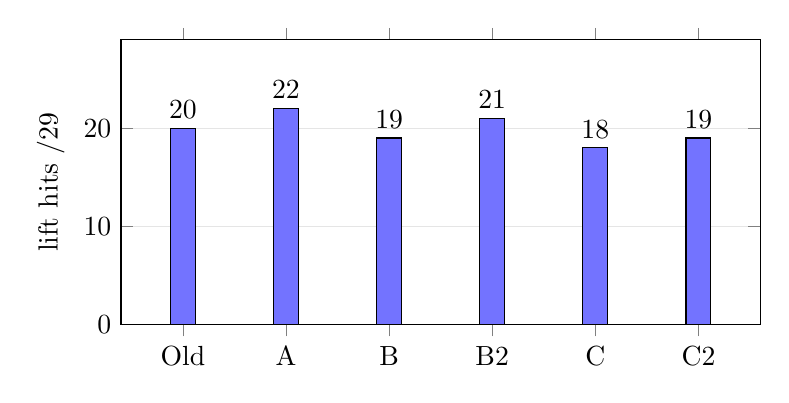
\begin{tikzpicture}
\begin{axis}[ybar, bar width=9pt, width=0.8\linewidth, height=5.2cm, ymin=0, ymax=29, ylabel={lift hits /29},
  symbolic x coords={Old,A,B,B2,C,C2}, xtick=data, nodes near coords, ymajorgrids, grid style={gray!20},
  enlarge x limits=0.12]
  \addplot[fill=blue!55] coordinates {(Old,20) (A,22) (B,19) (B2,21) (C,18) (C2,19)};
\end{axis}
\end{tikzpicture}
\caption{Lift (L-C) hits per teacher design at the default floor, amended query sets. With a floor sweep, B2 without
level choice reaches 24/29 at the same false-positive count.}
\end{figure}
\textbf{What we did.} \textbf{B2}: pyramid fallback in uncovered cells, SAM segments split into part/object/region levels, mask cache. \textbf{C2}: ViT-L/14's floor calibrated by quantile mapping over a neutral vocabulary (0.5222). Then a floor sweep over all designs and an inspection of FMGS's misses. Results: B2 21, C2 19 at the default floor.

\begin{center}\small
\begin{tabular}{@{}>{\raggedright\arraybackslash}p{0.162\linewidth}>{\raggedright\arraybackslash}p{0.582\linewidth}>{\raggedright\arraybackslash}p{0.204\linewidth}@{}}
\toprule
\textbf{Finding} & \textbf{Evidence} & \textbf{Consequence} \\
\midrule
A's lead is a floor effect & max over three groups raises every peak by \textasciitilde{}0.045 (absent objects too); A without the choice = 20; Old at floor 0.51 = 23 with the same false positives & the default should be decided with a calibrated floor \\
best trade-off: B2 without level choice & 24/29 with 2 of 6 absent objects firing & B2 flat is the strongest design measured \\
FMGS ``no candidate'' is not a floor problem & top-100 relevancies scattered 6–7.5 m apart, a third outside the camera volume & supervised-only baking and smoothing proposed \\
two ``absent'' objects fire everywhere & ceiling fan, recycling bin & the negative set needs a ground-truth check \\
\bottomrule
\end{tabular}
\end{center}
Reports: \code{semantic\_\allowbreak{}embedding\_\allowbreak{}report.tex} and \code{semantics\_\allowbreak{}primer.tex}.

\section{Lessons}
\begin{enumerate}
  \item \textbf{Pin everything and never let an install move torch.} Most early failures were version drift (nerfstudio/gsplat, pycolmap, OpenCV 5, numpy 2, timm). Every later install used \code{-{}-no-deps} and a constraints file.
  \item \textbf{Host problems look like software problems.} Kernel pinning, Secure Boot keys, suspend, RAM exhaustion during compiles and power cuts each cost hours; resumable steps with on-disk state turned interruptions into minor delays.
  \item \textbf{Silent failures are the dangerous ones}: integer course cells, the frame sign convention, a wrong marker length, SfM folds, a stalled time optimiser reporting success. Each now has an explicit check.
  \item \textbf{Measure before believing a limit.} The 6 GB training ``minimum'' was 2.4 GB with images on the CPU; the FMGS out-of-memory was allocator fragmentation, not size; A's gain was mostly the floor.
  \item \textbf{Ground truth needs checking too}: two of our own annotations were wrong, and two ``absent'' objects look present.
  \item \textbf{Keep a development set apart from the evaluation set}, and freeze the evaluation set before results.
\end{enumerate}
\section{Timeline}
\begin{center}\small
\begin{tabular}{@{}>{\raggedright\arraybackslash}p{0.121\linewidth}>{\raggedright\arraybackslash}p{0.853\linewidth}@{}}
\toprule
\textbf{Date} & \textbf{Step} \\
\midrule
25 Jul & Feasibility and first install on the 4 GB laptop; example flight runs \\
2 Aug & Clean rebuild with \code{install\_\allowbreak{}figs.sh}; four host faults fixed \\
6 Aug & First own capture-to-flight on the RTX 2080 (1 h 40 min) \\
7 Aug & \code{figs\_\allowbreak{}pipeline.py}; repository created \\
27 Sep & Galley phases 0–3 (job queue, splat page, course editor); SV-Net pipeline started \\
28 Sep – 1 Oct & intellisense08 bring-up; SV-Net gate (pipeline works, student does not fly); drone model; ribbon UI \\
3–4 Oct & splat view, keyboard flying, video upload, Google Drive import \\
5 Oct & Semantics phases 0–3 gated in one day; FMGS written \\
6 Oct & FMGS gate passed; Claude Code on the host; Phase 5 evaluation, power cuts, frozen sets, results \\
7 Oct & diagnostic, ground-truth check, variants A/B/C \\
8 Oct & A merged as default; B2, C2, floor sweep; reports \\
\bottomrule
\end{tabular}
\end{center}
\end{document}
